%!TEX root = ../../thesis.tex

ATLAS is a general purpose particle detector designed to probe hadron-hadron collisions, 
from precise measurements of \ac{SM} predictions to searches for new physics.
As such, it was designed to achieve a good performance in the reconstruction of all 
physics objects interacting with the detector (electrons, muons, photons and jets), and 
to infer the existence of non-interacting particles through transverse momentum imbalance.
A good vertex resolution was needed for jet flavour tagging and the high pile-up 
environment expected at the \ac{LHC}. Other requirements included a fast trigger system 
to select interesting events to record.
%, and the ability to function in an environment with large radiation doses.

The design of ATLAS exhibits cylindrical and forward-backward symmetries with the nominal 
interaction point at the centre.\footnote{
	ATLAS uses a right-handed coordinate system with its origin at the nominal 
	interaction point. The $x$-axis points to the centre of the \ac{LHC} ring, the 
	$y$-axis points upwards, and the $z$-axis points along the beam line. Positions and 
	directions within the detector are given in spherical coordinates $(r, \theta, \phi)$ 
	where $r$ is the radial distance, $\theta$ is the polar angle and $\phi$ is the 
	azimuthal angle. Usually the polar angle is converted to pseudorapidity 
	$\eta = -\ln\tan(\theta/2)$. The distance between two positions in $\eta\mhyphen\phi$ 
	space is $\Delta R = \sqrt{\Delta\eta^2 + \Delta\phi^2}$.
	Observables labelled ``transverse'' are projected into the $x\mhyphen y$ plane.
} 
The three detector sub-systems (tracking, calorimetry and the muon spectrometer) 
follow a consistent design of a central barrel with end-caps at both ends, giving a high 
degree of hermeticity (see \Figure~\ref{fig:atlas_whole}). Barrel components are arranged 
on concentric cylinders around the beam axis, while end-cap components are on disks 
perpendicular to the beam axis.

\begin{figure}
	\includegraphics[width=\textwidth]{tex/experiment/atlas_whole}
	\caption{Cut-away view of the ATLAS detector \cite{ATLAS-detector}. It has a height 
	of \unit{25}{\metre}, a length of \unit{44}{\metre} and weighs 7000~tonnes.}
	\label{fig:atlas_whole}
\end{figure}

\Figure~\ref{fig:atlas_wedge} shows how different particles interact with the various 
parts of the detector. Next to the beam pipe is the inner detector which precisely tracks 
the trajectories of charged particles. Then there are the electromagnetic and hadronic 
calorimeters which absorb and measure the energy of interacting particles. Since muons are
minimum ionising particles, they survive the calorimeters and are tracked by the muon 
spectrometer. Superconducting solenoid and toroid magnets provide magnetic fields to the 
inner detector and muon spectrometer respectively, allowing the momenta of charged 
particles to be measured from the curvature of their tracks.

\begin{figure}
	\includegraphics[width=\hugefigwidth]{tex/experiment/atlas_wedge}
	\caption{Schematic cross-sectional view of the ATLAS detector to show how a variety 
	of different particles would interact with the sub-detectors on its trajectory from 
	the interaction point. ATLAS Experiment \copyright\xspace 2013 CERN.}
	\label{fig:atlas_wedge}
\end{figure}

\subsection{Tracking}

\begin{figure}
	\includegraphics[width=0.55\textwidth]{tex/experiment/id_whole}
	\hfill
	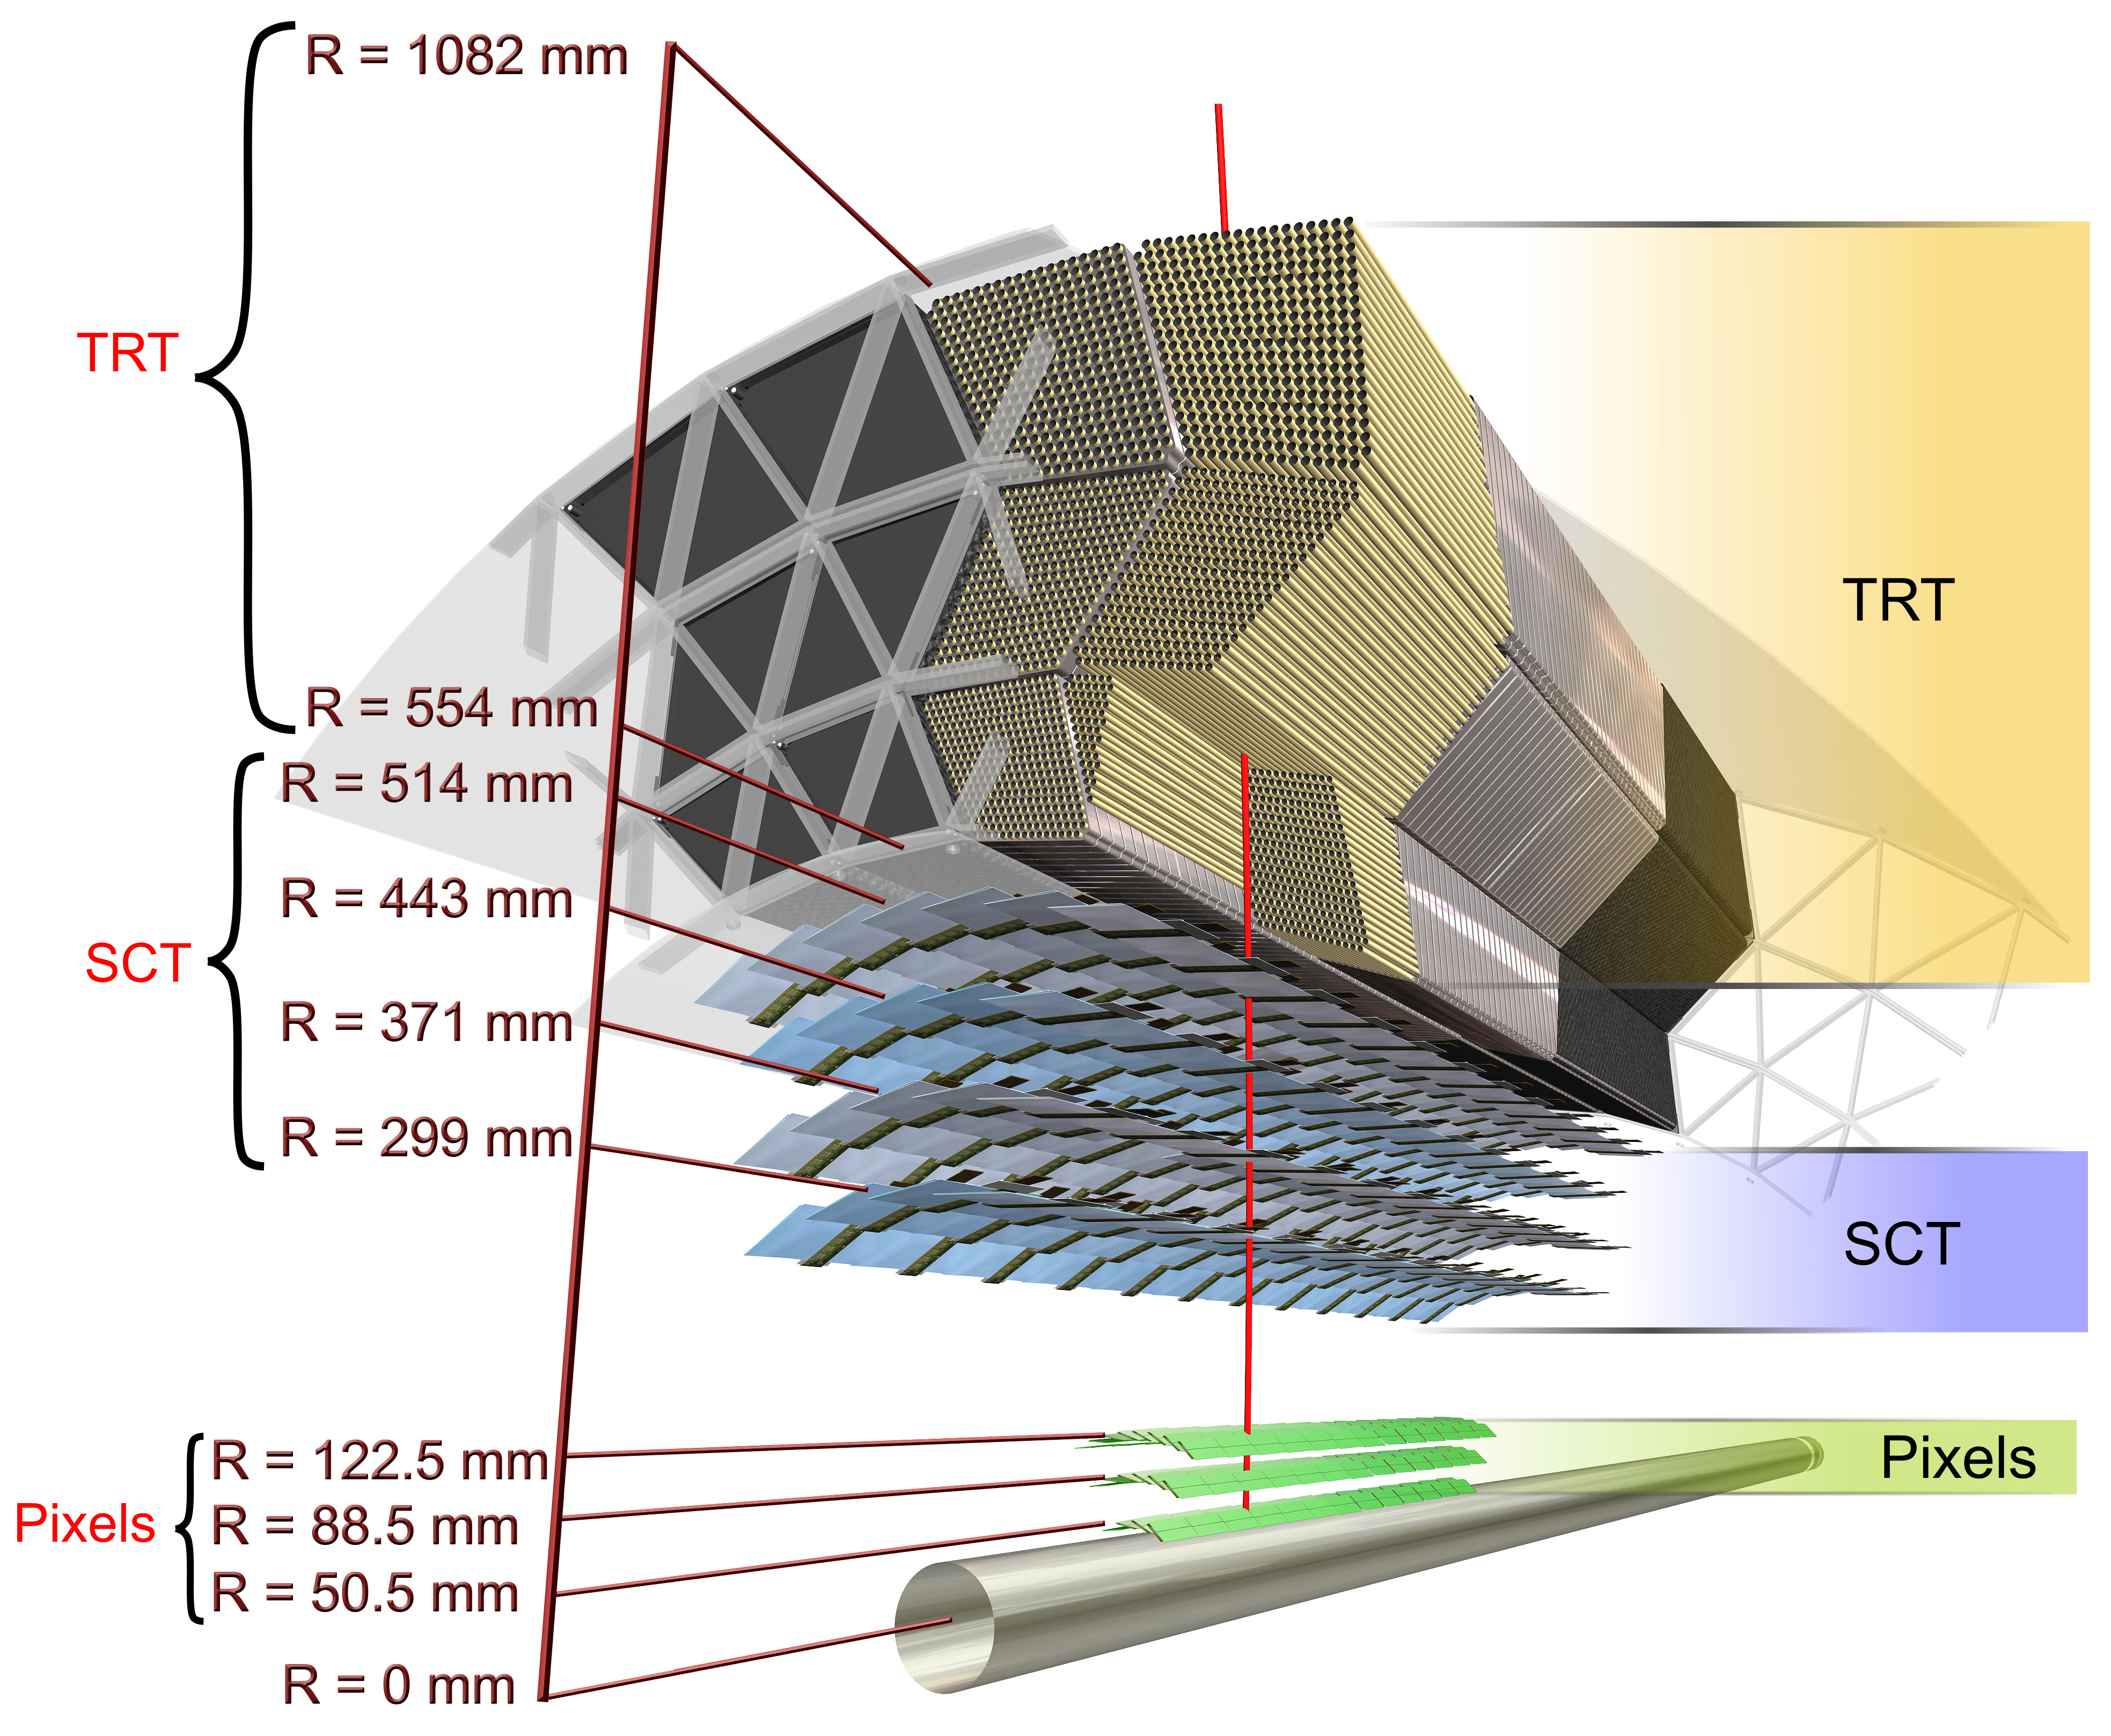
\includegraphics[width=0.44\textwidth]{tex/experiment/id_wedge}
	\caption{The ATLAS inner detector: (left) cut-away view and (right) cross-sectional 
	view showing a trajectory through the three sub-detectors \cite{ATLAS-detector}. The 
	inner detector has a length of \unit{6.2}{\metre} and a radius of \unit{1.1}{\metre}. 
	The beam pipe has radius \unit{29}{\milli\metre}.}
	\label{fig:inner_detector}
\end{figure}

Pattern recognition algorithms are used to precisely track the trajectories of charged 
particles through the \ac{ID}, shown in \Figure~\ref{fig:inner_detector}. The \ac{ID} is 
immersed in a \unit{2}{\tesla} solenoidal magnetic field, which enables the momentum of a 
particle to be measured from the curvature of its track. Momentum and vertex measurements
both require an excellent spatial resolution, which is achieved through fine detector 
granularity. The \ac{ID} covers the region $\mods{\eta} < 2.5$ and consists of three 
complementary sub-detectors:
\begin{description}
	\item[Pixel detector] \hfill \\
	The pixel detector is installed in three layers closest to the beam pipe, and 
	therefore requires the highest granularity to deal with the large particle fluxes.
	It consists of more than 80 million silicon pixels, each of size 
	\unit{$50 \times 400$}{\micro\metre\squared} and thickness \unit{250}{\micro\metre}. 
	The intrinsic accuracy is \unit{10}{\micro\metre}$\,\times\,$\unit{115}{\micro\metre} 
	in $r\phi \mhyphen z$ ($r\phi \mhyphen r$) space for the barrel (end-cap).

	A silicon particle detector consists of a reverse-biased p-n junction. When a charged
	particle passes through the depletion region it creates an electron-hole pair, which 
	travel to the respective electrodes and produce a signal current.
	\item[\ac{SCT}] \hfill \\
	The \ac{SCT} features 15,912 silicon strip sensors, each consisting of 770 strips 
	with a pitch of \unit{80}{\micro\metre} and a length of \unit{6}{\centi\metre}. Pairs 
	of sensors are sandwiched together (forming modules) with a stereo angle of 
	\unit{40}{\milli\radian}, which enables the $z$-coordinate of the hit to be measured. 
	There are four (nine) layers of modules in the barrel (end-cap), which ensures that 
	each track passes through four modules. 
	The intrinsic accuracy is \unit{17}{\micro\metre}$\,\times\,$\unit{580}{\micro\metre} 
	in $r\phi \mhyphen z$ ($r\phi \mhyphen r$) space for the barrel (end-cap).
	\item[\ac{TRT}] \hfill \\
	The \ac{TRT} features 370,000 drift chambers (straws) which simultaneously function 
	as a straw tracker to enhance particle tracking and as a transition radiation 
	detector to aid electron identification. Straws are aligned with the beam pipe in the 
	barrel and radially in the end-caps. The \ac{TRT} covers the region 
	$\mods{\eta} < 2.0$.

	Each \unit{4}{\milli\metre} diameter straw has a 
	Kapton\textsuperscript{\circledR}\xspace wall with a conductive coating, which 
	acts as a cathode at \unit{$-1530$}{\volt}, and a central tungsten wire anode. The 
	straws are filled with a xenon-based gas mixture that is ionised by a traversing 
	charged particle. The negative ions drift to the anode and produce a signal current. 
	The drift time is used to measure the impact parameter of the incident charged 
	particle relative to the anode and, since a track typically traverses 36 straws, this 
	collective information yields an intrinsic accuracy of \unit{130}{\micro\metre} in 
	$r\phi$ (much smaller than the straw diameter). However, tracking information 
	parallel to the straw is lost.

	The layers of straws are interleaved with polypropylene radiator fibres or foils, and 
	the changes in refractive index cause charged particles to emit X-ray transition 
	radiation (TR). The TR is absorbed by the xenon gas in the straws; TR signals are 
	distinguished from tracking signals with a higher threshold. Since the probability of 
	TR is proportional to the particle's $\gamma$-factor, for a given energy lighter 
	particles produce more TR than heavier particles. This aids electron-pion 
	discrimination.
\end{description}

\subsection{Calorimetry}

\begin{figure}[b]
	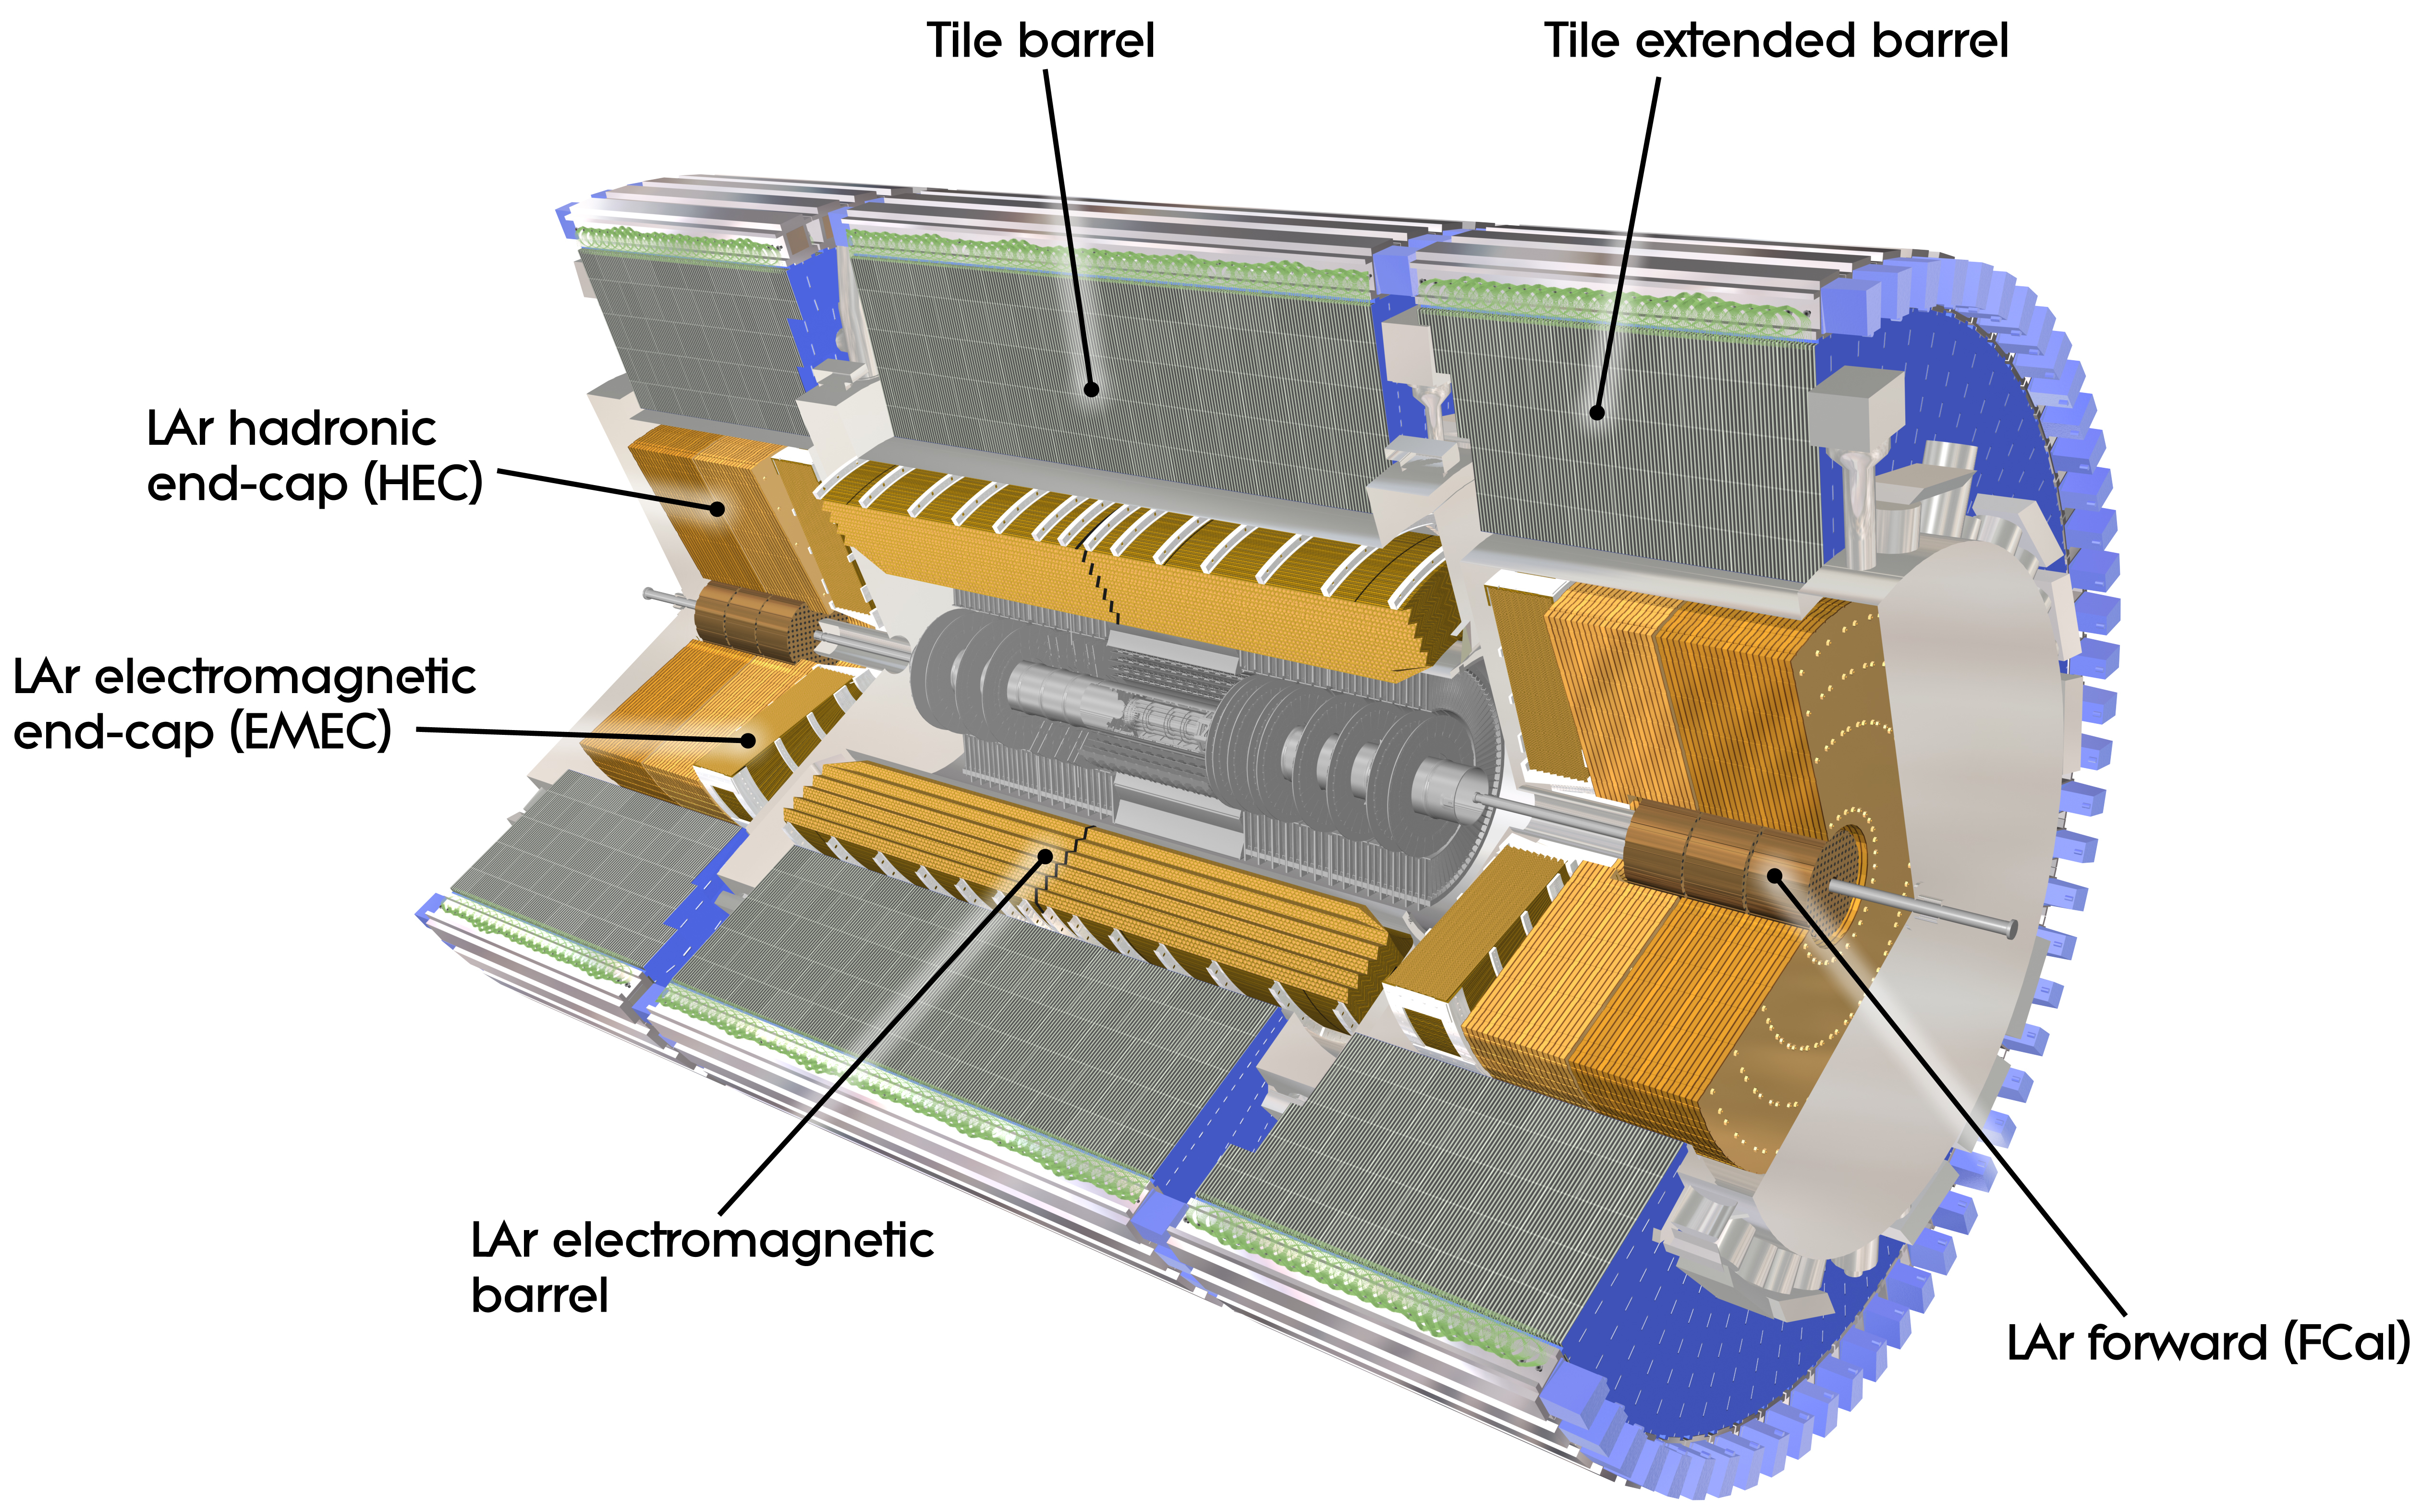
\includegraphics[width=\largefigwidth]{tex/experiment/calo_whole}
	\caption{Cut-away view of the ATLAS calorimeter system \cite{ATLAS-detector}.}
	\label{fig:calorimeters}
\end{figure}

\subsection{Muon spectrometer}

\begin{figure}
	\includegraphics[width=\largefigwidth]{tex/experiment/ms_whole}
	\caption{Cut-away view of the ATLAS muon spectrometer \cite{ATLAS-detector}.}
	\label{fig:muon_spectrometer}
\end{figure}

\subsection{Trigger and data acquisition}

